\documentclass[10pt,twocolumn]{article}
\usepackage[a4paper, left=1.5cm, right=1.5cm, top=2cm, bottom=2cm]{geometry}
\usepackage[T1]{fontenc}
\usepackage[utf8]{inputenc}
\usepackage[italian]{babel}
\usepackage{amsmath}
\usepackage{titling}
\usepackage{caption}
\usepackage{graphicx}
\usepackage{float}
\usepackage{relsize}
\usepackage{amsmath}
\usepackage{sectsty}
\usepackage{ragged2e}
\usepackage{circuitikz}
\usepackage{booktabs}
\usepackage{enumitem}
\usepackage{tikz}
\usepackage{physics}
\usepackage{xcolor}
\usepackage[most]{tcolorbox}
\usepackage{tikz-3dplot}
\usepackage{tikz}
\usepackage{ragged2e}
\usepackage{siunitx}
% \usepackage{booktabs}
\usepackage[colorlinks=true, linkcolor=black]{hyperref}  %per rendere l'indice genrale "interattivo"
\usepackage{enumitem}  %distanza degli itemize
\setlist[itemize]{itemsep=4pt, parsep=1pt}
\newtcolorbox{nota}{
  blanker,
  before skip=1em,
  after skip=1em,
  left=1em,
  borderline west={1pt}{0pt}{black},
  fontupper=\itshape,
  before upper={\noindent\textbf{Nota}:\quad}
}



\begin{document}
\justifying
	\title{\textbf{Misura della curva volt-amperometrica di una lampadina a filo di tungsteno}}
	\author{Brusini Alessio \hspace{0.7cm} Ferrari Carola \hspace{0.7cm} Mirolo Manuele \hspace{0.7cm} Stroili Emanuele}
	\date{14 Ottobre 2025}
	\maketitle
	\newgeometry{left=3cm, right=3cm, top=4cm, bottom=4cm}
	\onecolumn
	\tableofcontents
\vspace{3cm}
	\begin{abstract}
		\centering
		\large
    L'esperimento consiste nell'ottenere la curva volt-amperometrica di una 
    lampadina a filamento, partendo da tensioni basse fino alla fusione del 
    tungsteno. L'obiettivo è verificare l'andamento non ohmico della resistenza
    interna della lampadina, 
       
	\end{abstract}

	\newpage
\restoregeometry
\twocolumn

\section{Apparato sperimentale}
\subsection{Misura per bassi voltaggi}
Per ottenere la misura a bassi voltaggi si costruisce un circuito composto da:
\begin{itemize}
    \item Generatore di corrente continua
    \item Resistenza 
    \item Voltmetro
    \item Amperometro
    \item Fotodiodo
    \item Lampadina con tensione di funzionamento 6V
\end{itemize}
\begin{center}
\begin{circuitikz}[american]
    
    % Generatore di corrente continua variabile a sinistra
    \draw (0,0) to[battery1, invert, l=$V$] (0,3);
    
    % Resistenza in alto
    \draw (0,3) to[R, l=$R$] (3,3);
    
    % Lampadina a destra
    \draw (3,3) to[lamp, l=$L$] (3,0);
    
    % Amperometro in basso
    \draw (0,0) to[rmeter, t=A] (3,0);
    
    \draw (3,2) to[short] (4.5,2) 
    % Voltmetro in parallelo alla lampadina
    to[rmeter, t=V] (4.5,1)
    to[short] (3,1);
\end{circuitikz}
\end{center}

\section{Procedimento di misura}
La misura si svolge in due fasi: nella prima si prendono misure più fitte
per poter apprezzare le oscillazioni di corrente. A questo scopo è necessario
introdurre una resistenza nel circuito da utilizzare come partitore di tensione.
Inoltre, nella prima fase, ci si serve di un fotodiodo per poter captare la 
flebile luminescenza della lampadina, non visibile univocamente a occhio nudo.\\
Nella seconda fase si prendono dati meno fitti, perciò si rimuovono la 
resistenza e il fotodiodo dal circuito, non più necessari nella misura.

\section{Dati}
\begin{table}[H]
    \begin{minipage}{0.5\textwidth}
        \centering
        \caption*{}
        \label{tab:temp2}
        \begin{tabular}{|r|r|}
            \hline
            Tensione(V) & Corrente (A) \\ \hline
            0 & 17.2 \\ \hline
            30 & 17.2 \\ \hline
            60 & 17.2 \\ \hline
            90 & 17.2 \\ \hline
            120 & 17.1 \\ \hline
            150 & 17.1 \\ \hline
            180 & 17.1 \\ \hline
            210 & 17.2 \\ \hline
            240 & 17.1 \\ \hline
            270 & 17.1 \\ \hline
            300 & 17.2 \\ \hline
            330 & 17.2 \\ \hline
            360 & 17.2 \\ \hline
            390 & 36.9 \\ \hline
            420 & 36.8 \\ \hline
            450 & 36.7 \\ \hline
            480 & 36.6 \\ \hline
            510 & 36.5 \\ \hline
            540 & 36.4 \\ \hline
            570 & 36.4 \\ \hline
            600 & 36.3 \\ \hline
            630 & 36.1 \\ \hline
            660 & 36.1 \\ \hline
            690 & 36.0 \\ \hline
            720 & 35.9 \\ \hline
            750 & 35.9 \\ \hline
            780 & 35.8 \\ \hline
            810 & 35.8 \\ \hline
            840 & 35.7 \\ \hline
            870 & 35.7 \\ \hline
            900 & 35.7 \\ \hline
            930 & 35.7 \\ \hline
            960 & 35.6 \\ \hline
            990 & 35.6 \\ \hline
            1020 & 35.5 \\ \hline
        \end{tabular}
    \end{minipage}
\end{table}

\twocolumn

\section{Grafici}
\begin{figure}[H] % [h] = here, posizione approssimativa
  \centering
  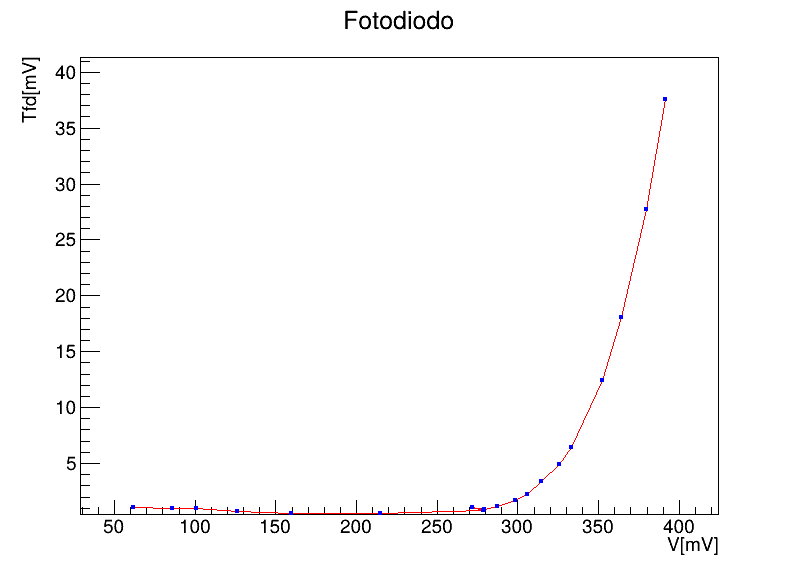
\includegraphics[width=0.5\textwidth]{curva_voltammetrica/fotodiodo.png} % o .png, .pdf, ecc.
  \label{fig:esempio}
\end{figure}
\end{document}